%
%\documentclass[11pt]{uwthesis}
%\usepackage[pdftex]{graphicx}
%%\usepackage{plain} % references
%%\usepackage{namedplus}
%\usepackage{jneurosci}
%\usepackage{booktabs}
%\usepackage[usenames,dvipsnames]{color}
%\usepackage{rotating}
%\usepackage{stmaryrd}
%\usepackage{textcomp}
%\usepackage[margin=10pt,font=small,labelfont=bf, labelsep=endash]{caption}
%
%
%% strain names
%\def\sWT{\emph{WT}~}
%\def\sfullWT{C57B/6J~}
%\def\sRhoKO{\emph{Rho$^{-/-}$}~}  %strain name  {\emph{Rho$^{tmLem}$}}
%\def\sRhoHet{\emph{Rho$^{+/-}$}}  %strain name
%\def\sStoA{Tg(Rho/${\rm{S}\shortrightarrow \rm{A}}$)~}	%strain name
%\def\sTtoA{Tg(Rho/${\rm{T}\shortrightarrow \rm{A}}$)~}
%\def\sArrKO{\emph{Arr1$^{-/-}$}}
%\def\sArrHet{\emph{Arr1$^{+/-}$}}
%\def\sRKKO{\emph{GRK1$^{-/-}$}}
%\def\sRKHet{\emph{GRK1$^{+/-}$}}
%
%\def\sGCAP{\emph{GCAP$^{-/-}$}}
%\def\GCAP{GCAP$^{-/-}$}
%
%\def\OneP{Tg(Rho/S388)}
%
%
%% Proteins
%\def\Rho{Rho~}
%\def\TtoA{T$\shortrightarrow$A~}	%protein name
%\def\StoA{S$\shortrightarrow$A~}
%
%\def\CVa{CV$_{area}$~}
%\def\CVarea{CV$_{area}$~}
%\def\Mg{Mg$^{2+}$~}
%\def\Ba{Ba$^{2+}$~}
%\def\Cd{Cd$^{2+}$~}
%\def\Ca{Ca$^{2+}$~}
%\def\Na{Na$^+$~}
%\def\K{K$^+$~}
%\def\Cl{Cl$^-$~}
%\def\uM{$\mu$M~}
%\def\s{$\sec^{-1}$~}
%\def\pho{${\rm photons}\,\mu {\rm m}^{-2}\sec$~}
%\def\phos{${\rm photons}\,\mu {\rm m}^{-2}$~}
%\def\Lphos{photoisomerizations$/$sec$/$L cone}
%\def\CO2{CO$_2$~}
%\def\O2{O$_2$~}
%\def\on{{\sc on}~}
%\def\off{{\sc off}~}
%\def\onoff{{\sc on/off}~}
%\def\bi{\begin{itemize}}
%\def\ei{\end{itemize}}
%\def\i{\item}
%\def\be{\begin{enumerate}}
%\def\ee{\end{enumerate}}
%\def\tpeakratio{$t_{peak, \sigma^2} / t_{peak, m}$}
%\def\varwidth{$w_{\sigma^2}$}
%
%% parameters
%\def\Kme{$K_{P}$~}
%\def\Kmt{$K_{M-T}$~}
%\def\Trh{$T_{Rh}$~}
%\def\Ns{$N_s$~}
%\def\Kmr{$K_{M-Rh}$~}
%
%%
%%
%%
%%\begin{figure}[tb!]
%%\begin{center}
%%\includegraphics[scale=0.5]{Fig_SvTX.eps}
%%\caption[TOCcaption]
%%{<caption>}
%%\label{Fig_SvTX}
%%\end{center}
%%\end{figure}
%%
%%
%%

%\begin{document}
%\textpages
%%%%

\chapter{Reproducibility of Single-Photon Responses Reflects Tightly Controlled GPCR activity}
\label{chap:repro}
\baselineskip 24pt

%Anthony Azevedo, Dan Tranchina, Fred Rieke


\section{Summary}
% shorten, too much
The rod phototransduction cascade underlies sensitive visually guided behavior by encoding the arrival of single photons and their activation of individual molecules of rhodopsin, a G protein coupled receptor.  A G protein-mediated cascade then amplifies receptor activity, resulting in remarkably reproducible fluctuations in rod outer-segment current, offering an elegant system to study and quantify mechanisms that transduce signals originating from single GCPRs.  Here, we offer a rationale for a simplified model of stochastic receptor activity and transduction cascade, and we present an approach for evaluating how well the model, for a given set of parameter values, can account for measured properties of ensembles of isolated single-photon responses.  We find that the model is well-constrained by experimental data, and that the constraints suggest that the transduction cascade responds linearly to receptor activity, and thus that response reproducibility reflects tightly controlled receptor activity.  

\section{Introduction}

Visually-guided behavior of vertebrates in near-darkness requires rod photoreceptors to detect and signal the arrival of single photons reliably \cite{Field:2005fa}.  The response to single photons is accomplished by amplifying the activity of a single molecule of rhodopsin, a G protein coupled receptor (GPCR), leading to a brief, detectable reduction in the current into the rod outer segment .  This process provides an unparalleled opportunity to study how signals originating from single G-protein coupled receptors (GPCRs) are controlled \cite{Arshavsky:2002ik}.  Though the unitary response reflects the activity of a single active rhodopsin, the resulting electrical responses have long been known to show much less variability in either amplitude or kinetics than might be expected \cite{Baylor:1979wd}.  

The initial transduction steps are confined to the surface of membrane discs in the rod outer segment:  rhodopsin catalytically activates the G-protein transducin, which in turn activates a cGMP phosphodiesterase, PDE6 \cite{Wensel:2008ib}.  Phosphodiesterase then hydrolyzes cGMP, perturbing its cytosolic concentration and causing cGMP-gated channels in the outer segment membrane to close, thus coupling the activity on the disc to the plasma membrane current.  Rhodopsin activity shuts off through canonical GPCR desensitization reactions of phosphorylation and arrestin binding, PDE hydrolysis slows with transducin GTPase activity, and the current response recovers as cGMP is resynthesized by guanylyl cyclase (reviewed by \cite{Arshavsky:2002ik}).  Calcium feedback to the guanylyl cyclase contributes to speed response recovery kinetics \cite{Burns:2002un}.

As a system, this signaling scheme produces responses that show much less variability than the typical first-order kinetics of other single-molecule processes, such as the charge flowing through an ion channel during a single opening. 
This reproducibility could, in principle, be explained either by low variability in the number of transducin molecules activated during the receptor lifetime or by nonlinearities in the transduction process that reduce the impact of higher variation in transducin activation.  That is, the more variable the number of transducins activated, the stronger the nonlinear mechanisms would have to be to explain the reproducible nature of responses to single photons.   Here, we develop a simple model to explore the trade-offs between sources of variability and mechanisms capable of suppressing this variability.

\section{Methods}
\label{meth:repro}

\subsection{Suction-electrode recordings}

Suction electrode recordings of mouse rods were made as described, and single-photon responses were isolated based on their amplitude.   Data used here to constrain models have been previously reported, with the exception of single-photon responses from \sGCAP\ and \sRhoHet/\OneP lines \cite{Azevedo:2011ev,Doan:2006jr,Doan:2009jq}.  For measuring features of ensemble variance across cells within a given line, responses are normalized to the peak amplitude of the cell average, and response time course is normalized to the time-to-peak.  
%Values of variance width are then reported in relation to the mean.

We seek to identify likely characteristics of receptor kinetics and transduction that explain response properties across different mouse strains.  If no genetic manipulations are made to change the cascade, a model should be able to account for response properties in lines with mutations that only affect receptor activity in well-described ways.  To this end, we use responses from \sRKHet, Tg(Rho/0P), and \OneP/\-\sRhoKO~rods \cite{Chen:1999tp,Mendez:2000vh,Doan:2009jq,Doan:2006jr}.  To control for effects of transgenic expression rhodopsin mutants, we also crossed \sWT\  and \OneP/\sRhoKO\ lines, and recorded from \sRhoHet/\OneP\ rods that express both normal and mutated rhodopsin. 

Likewise, an accurate model of receptor activity will account for responses in rods with mutations that do not affect rhodopsin kinetics.  Knockout of guanylyl cyclase accelerating protein (GCAP) removes calcium sensitivity of the cyclase and results in prolonged responses with larger amplitudes than \sWT\  rods, but should not affect activity on the disk.  Likely parameters are those that can account for ensemble statistics in both \sGCAP\ and \sWT\ rods simultaneously.

\subsection{Models}
Below, we define parameters that govern a reduced model of the phototransduction cascade.  We constrain the model to reflect the average properties of single-photon response ensembles, and evaluate parameters for their ability to replicate the properties of trial-to-trial variation in experimental data.  Specifically, likely models will simulate responses with the following features (Fig.~\ref{fig:features}).
First, the overall variability is low; the coefficient of variation of response area, \CVarea, calculated as the standard deviation of response area divided by the mean, is in the range of $\sim0.3$-$0.35$ for normal mouse rods at 37\textcelsius, indicating that the reduction in charge influx varies by only $\sim35\%$.  Secondly, responses are less variable during the rising phase than during the falling phase, such that the response variance peaks later than the mean.  The ratio of the time-to-peak of the variance to the time-to-peak of the mean for \sWT\ mice is around $\sim1.8$.  The variance also has a characteristic width, \varwidth, measured at half height.  One can think of these features as analogous to minimal parameters of other functions: a height (\CVa), a width (\varwidth), and an offset (\tpeakratio).  

\begin{figure}[h]
\begin{center}
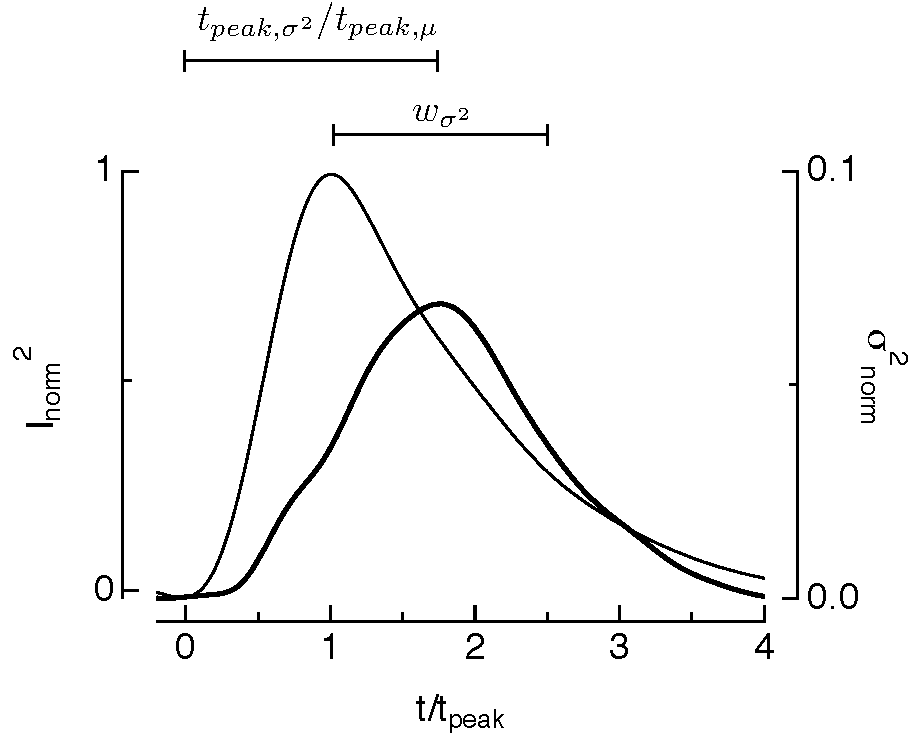
\includegraphics[width=4in]{params.pdf}
\caption[Features used in likelihood analysis]
{Features used in likelihood analysis. Data are from WT mice at 37\textcelsius.  The normalized mean-squared response (thin trace, left axis) and single-photon response variance (thick trace, right axis) are plotted as a function of $t/t_{peak, \mu}$, normalized to $t_{peak,\mu}$, the time-to-peak of the mean.
}  
\label{fig:features}
\end{center}
\end{figure}

In this study, we avoid detailed mechanistic descriptions in the service of exploring a few key parameters hypothesized to control properties of the response - simplifications which we justify below.  Though intended to represent the effects of known mechanisms, we maintain a level of abstraction meant to schematize the cascade components.  

\subsubsection{Stochastic model for rhodopsin activity}

We model receptor inactivation as a series of multiple shutoff steps, such that rhodopsin lifetime is effectively a sum of several sequential random, first-order lifetimes.  The model receptor activity is specified by the number of shutoff steps, the reduction of activity produced by each inactivation step; and by the time scale of inactivation.  Rhodopsin activity could alternatively be controlled by feedback, but studies have shown that Ca$^{2+}$-mediated feedback to rhodopsin is minimal during the single-photon response \cite{Burns:2002un,Makino:2004gc,Sampath:2005ba,Chen:2010hk}, and we chose not to include it in our model. 

\begin{figure}[tb!]
\begin{center}
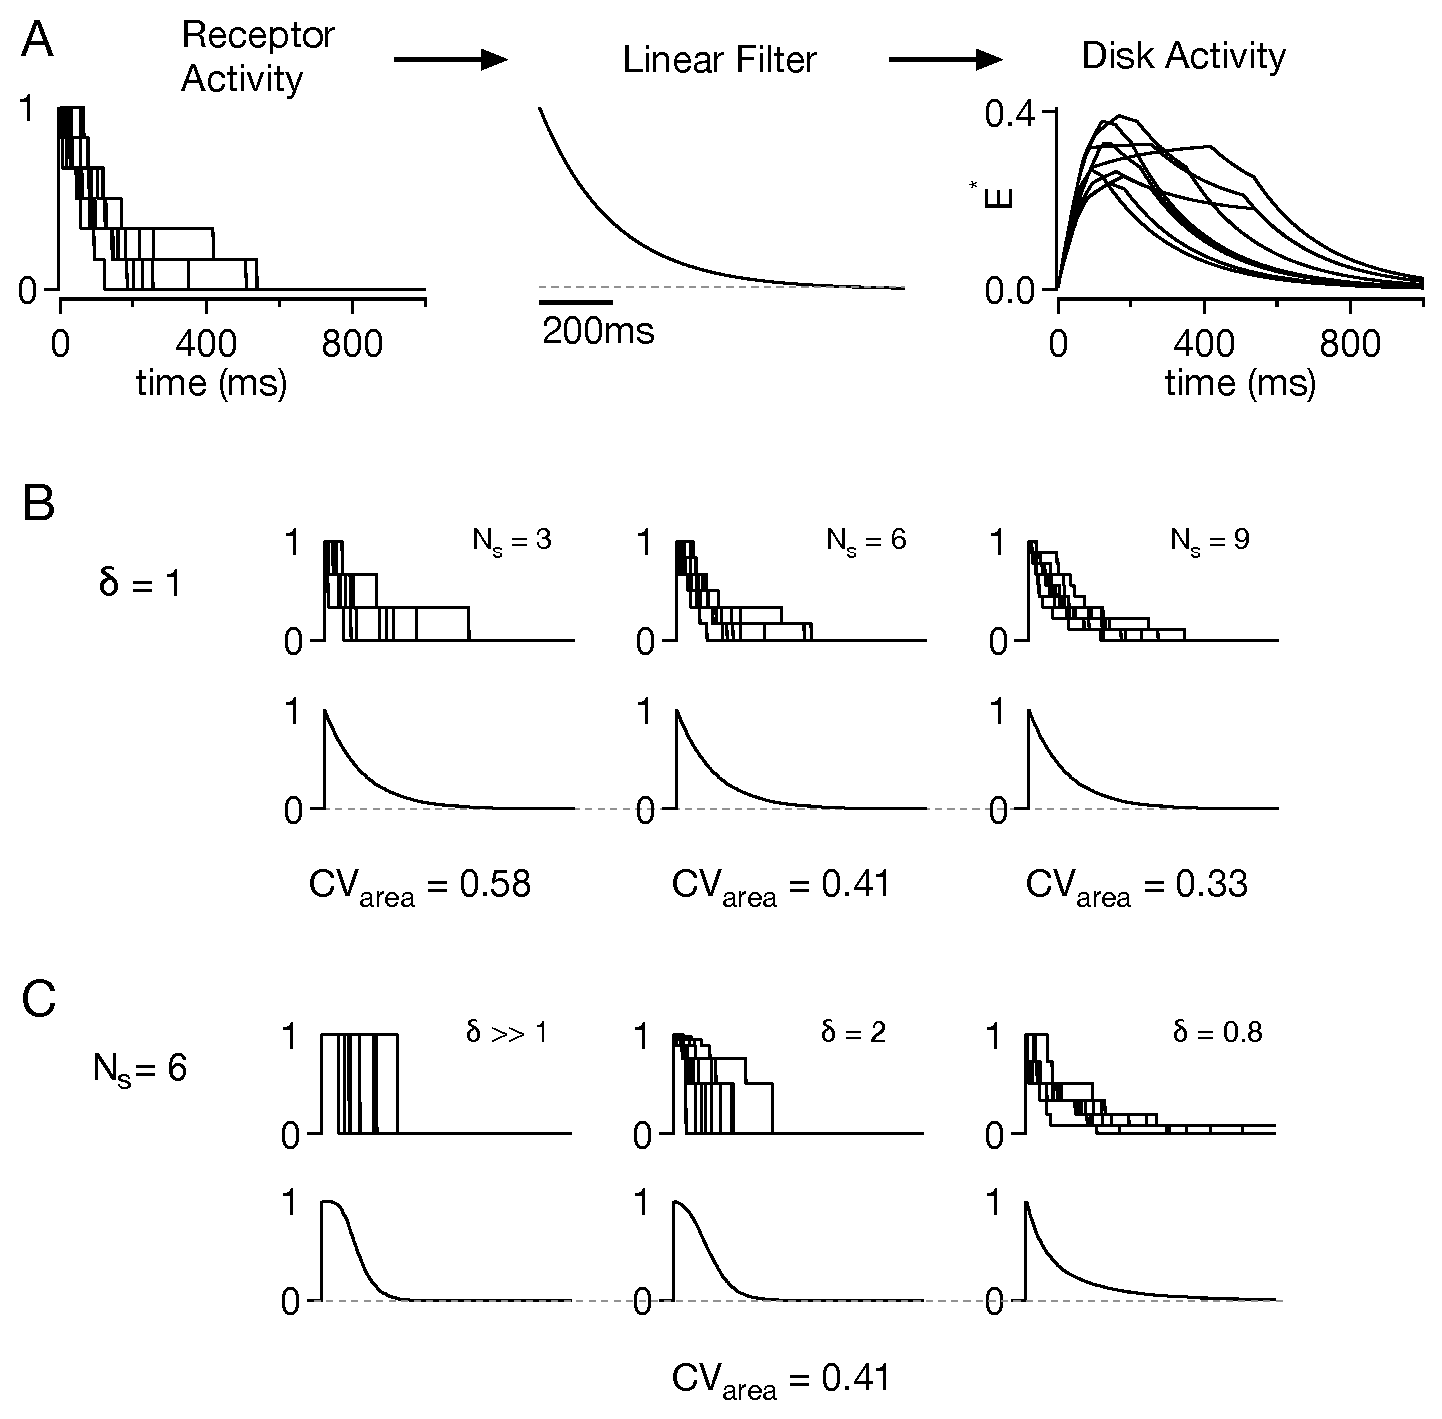
\includegraphics[scale=0.55]{ModelParams2.eps}
\caption[Parameters of stochastic receptor activity: \Ns, $\delta$, \Trh.]
{Parameters of stochastic receptor activity: \Ns, $\delta$,  \Trh.
A) Receptor activity simulated according to the model parameters (here: \Ns$= 6$, $\delta=1$, \Trh$=150$ ms) gets convolved with a filter approximating the time scale of transducin inactivation (200 ms) to generate hydrolysis activity on the disk. The nine receptor trajectories generate the nine disk activity traces.  Alternatively, PDE activity can also be stochastically generated as described in the text.   
B) The parameter, $\delta = 1$, is held constant as the number of steps in receptor shutoff increase.  Nine traces in each panel.  The average of $N = 5000$ trajectories is unchanged with \Ns, whereas \CVa\ $\sim 1/\sqrt{N_s}$.  Time scale is arbitrary, set by \Trh.
C) The parameter, \Ns$ = 6$, is held constant as $\delta$ decreases.  \CVa$=1/\sqrt{N_s}$ is constant, but the shape of the average now depends on $\delta$.
}
\label{fig:rhparams}
\end{center}
\end{figure}

Rhodopsin catalytic activity is assumed to begin at time, $t = 0$, and proceeds through a series of $N_s$ steps (Fig \ref{fig:rhparams}B).  
Each step entails a reduction in rhodopsin's activity, given by $\Delta Rh_i$.  These steps were determined by dividing the interval [0,1] into geometric sections, $\Delta Rh_i$, where $\Delta Rh_{i+1} = (\delta^i) \Delta Rh_{i}$.  The initial step, $\Delta Rh_1$, will be set to ensure that the sum of all steps equals one (Fig \ref{fig:rhparams}B).  The final step inactivates the remaining activity.  Steps make equal drops when $\delta=1$ and $\Delta Rh_i = 1/N_s$.  This scheme for defining $\Delta Rh_i$ was chosen in order to model a wide range of reductions in activity with a single parameter, producing both step-like activity with a single transition ($\delta \gg 1$) and activity that quickly is reduced, creating a long tail ($\delta < 1$) (Fig \ref{fig:rhparams}C).  

The average rate, $k_i$, at which rhodopsin takes the next step is then determined by the activity level, $Rh = 1-\sum_i \Delta Rh_i$, such that the ratio of rate and receptor activity is constant for all steps.  At each point in time (here, sampled every millisecond), the next reduction in activity was made if a random number on interval [0, 1] was less than the rate per sampling period, $\Delta T$, for that step, $k_i/\Delta T$, a Bernoulli process.  This scheme ensures that both the average and the variance of the activity (area) across steps are constant, providing a minimum in the variance of integrated activity across multiple steps \cite{Hamer:2005ec}. 

The total average activity is represented by \Trh.  The most general definition of \Trh\ is the integral of the average receptor activity over time,  and is given in units of time because receptor amplitude is scaled to a maximum value of one.  This is a convenient definition when $\delta=1$ (the case when activity reduction is constant across steps) since the average response is a decaying exponential with time constant \Trh\ (Fig.~\ref{fig:rhparams}B).  When $\delta$ takes on different values, then \Trh\ still represents the average activity (integral), but the balance of activity can shift towards late or early times (Fig.~\ref{fig:rhparams}C)
% what do we read that will help to understand or relate the steps in Rhodopsin activity to things other than phosphorylation?

\subsubsection{Deterministic disk reactions}

In this study, we describe the set of reactions taking place on the disk simply as the effector activity, or disk activity, $E^*(t)$.  We model the response of $E^*(t)$ to an impulse of receptor activity as a deterministic, linear filter, described by an exponential decay (Fig \ref{fig:rhparams}A).  Effector activity thus represents the time-course of both transducin and its target, PDE
\cite{Chen:2000fv,ArshavskyVYu:1992dd}, as well as any delays between these reactions. The time course of this filter is well-constrained in the range $\sim 200-250$ ms \cite{Krispel:2006hh}. A deterministic response to receptor activity sets an upper bounds on variability introduced by rhodopsin.  That is, if in reality steps other than rhodopsin introduce significant trial-to-trial fluctuations, then any bound we can put on reproducible disk activity will mean even tighter control of rhodopsin desensitization.
The result of this operation is a set of simulated trajectories of $E^*(t)$, as shown to the right in Figure \ref{fig:rhparams}A. 

\subsubsection{Compression of disk activity}

Nonlinearities within the transduction cascade could reduce the sensitivity of the measured currents to variability in rhodopsin or transducin activity.  Such nonlinearities could take two general forms: (1) saturation of reactions on the membrane disc; (2) saturation of diffusible signals coupling disc activity to membrane channels.  We can take several approaches to incorporating such saturation into stochastic models.  The focus here is on simple empirical models that should encompass most forms of saturation. 

\begin{figure}[tb!]
\begin{center}
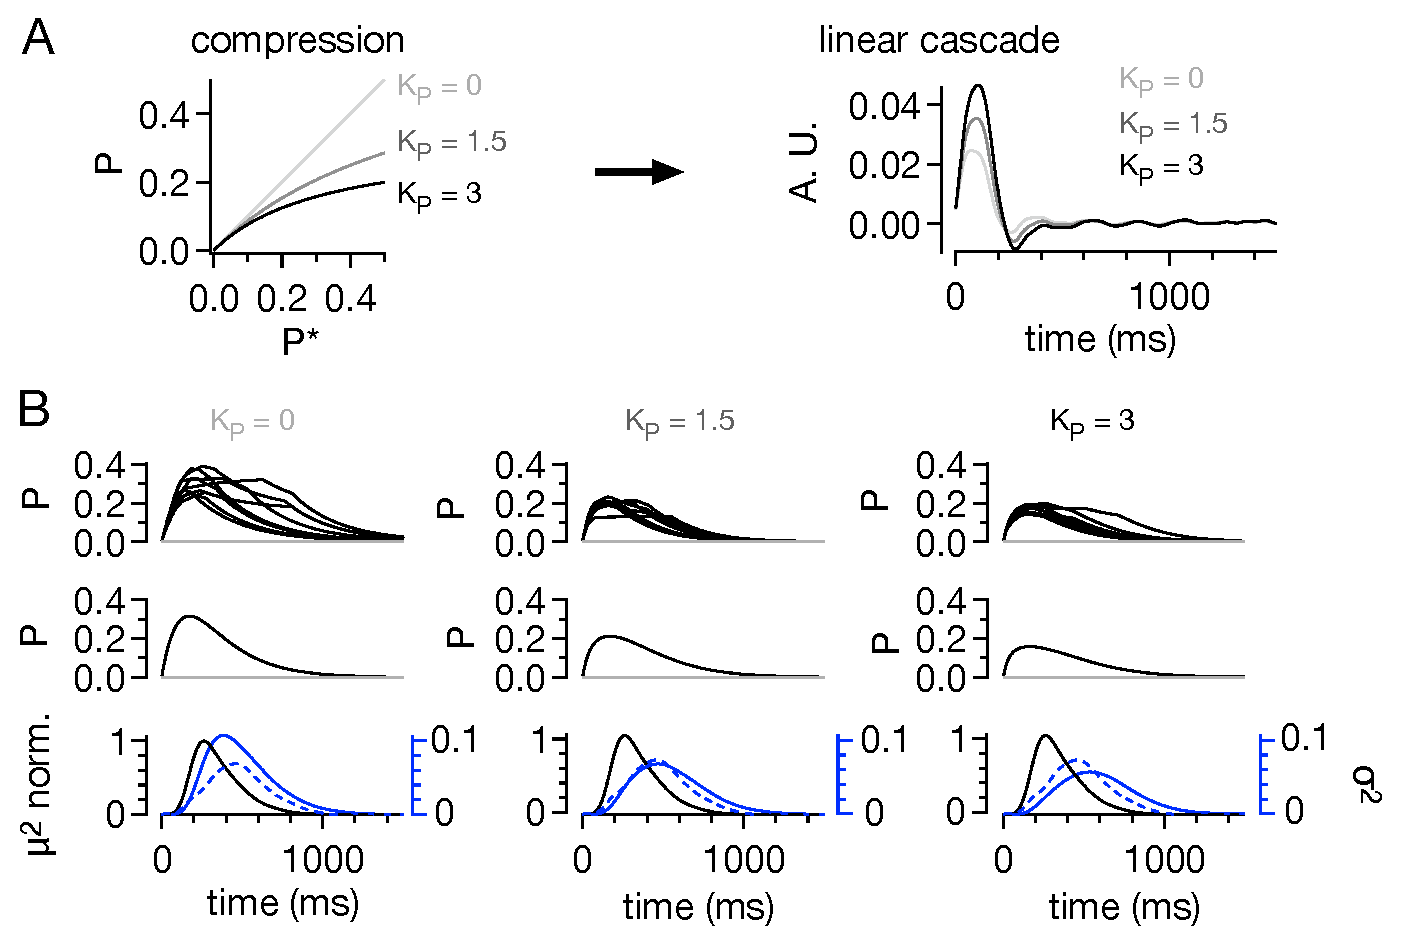
\includegraphics[scale=0.51]{EParams.eps}
\caption[Compression of effector activity (\Kme), and subsequent linear filtering.]
{Compression of effector activity (\Kme), and subsequent linear filtering.
A) Disk activity simulated as in Figure \ref{fig:rhparams} is then passed through a compressing nonlinearity (left, Eq.~\ref{eq:compr}).  Trajectories are then filtered with an impulse response.  
B) Simulated $E(t)$ trajectories with \Ns$=6$, \Trh$=150$ ms, $\delta=1$.  Larger values for \Kme\ compress responses, changing the shape of the average disk activity, $\bar{E}(t)$ (black traces).  C) Effector activity is filtered by the impulse response in (A) to produce a set of output responses (grey traces), with an average response $\mu(t)$ (black traces).  The impulse response in (A) is calculated such that $\mu(t)$ replicates the experimentally measured single-photon response.  D) Ensemble time-dependent variance is unconstrained and depends on the model (blue traces, right axes).  Note that variance is plotted on axes ten-fold smaller than the mean-squared activity (black trace, left axes).  Experimentally-measured variance (Fig.~\ref{fig:features}), is replotted in each panel for reference (blue dotted traces).
}
\label{fig:eparams}
\end{center}
\end{figure}

The effector activity $E^*(t)$ may not produce proportional changes in second messenger concentrations, as described below.  Instead, as $E^*(t)$ increases, for example, the effect of additional activity on on the cascade may decrease.  We model this reduced coupling as a Michaelis function, relating the effective activity on the disk, $E(t)$, to the effector time-course, $E^*(t)$:
\begin{equation} 
E(t) = \frac{E^*(t)}{1+K_{E} E^*(t)}.
\label{eq:compr}
\end{equation}
where \Kme\ has units of seconds and 1/\Kme\ in \s\ is the value of $E^*(t)$ that compresses hydrolysis in half.  This definition provides an intuitive connection between increasing values of \Kme\ and increasing compression.  Figure \ref{fig:eparams}B depicts the effect of this type of nonlinearity, where the amplitude of $E^*$ is compressed, and the average trajectory appears more rounded.  

A second form of compression represents the effect of exhaustion without replacement of the available components on the disk, either transducin or PDE.  Then the activity of $E(t)$ is affected by the cumulative $E^*(t)$, and the more is activated, the less is available:
\begin{equation} 
E(t) = \frac{E^*(t)}{1+\kappa \int_0^t E^*(t') \rm{d} t'}.
\label{eq:sat}
\end{equation}
The effect of this type of nonlinearity is to compresses both the amplitude and time course of $E^*(t)$, as shown in Figure \ref{fig:eparamssat}

\begin{figure}[tb!]
\begin{center}
\includegraphics[scale=0.51]{EParamsSat.eps}
\caption[Saturation of effector activity ($\kappa$), and subsequent linear filtering.]
{Saturation of effector activity ($\kappa$), and subsequent linear filtering.
A) Disk activity simulated as in Figure \ref{fig:rhparams} is then passed through a nonlinear saturation function that depends on the integrated $E^*(t)$ activity (left, Eq.~\ref{eq:sat}).  Trajectories are then filtered with an impulse response.  
B) Simulated $E(t)$ trajectories with \Ns$=6$, \Trh$=150$ ms, $\delta=1$.  Larger values for $\kappa$ compress responses, changing the shape of the average disk activity, $\bar{E}(t)$ (black traces).  C) Effector activity is filtered by the impulse response in (A) to produce a set of output responses (grey traces), with an average response $\mu(t)$ (black traces).  The impulse response in (A) is calculated such that $\mu(t)$ replicates the experimentally measured single-photon response.  D) Ensemble time-dependent variance is unconstrained and depends on the model (blue traces, right axes).  Note that variance is plotted on axes ten-fold smaller than the mean-squared activity (black trace, left axes).  Experimentally-measured variance (Fig.~\ref{fig:features}), is replotted in each panel for reference (blue dotted traces).
}
\label{fig:eparamssat}
\end{center}
\end{figure}
	
The output of the nonlinear relationships, the compressed trajectories, $E(t)$, represent the time-course of changes in second messenger concentration that will then determine the current response.  These trajectories incorporate all of the intervening reactions between receptor and second messenger, including any delays or saturation of components.

\subsubsection{Linear model relating current to changes in second messenger concentration.}
\label{meth:repro:cascd}
Thus far, a specific stochastically generated trajectory for receptor activity is passed through a linear filter representing disk activity, then acted on by compressive nonlinearities to generate fluctuations of second messenger, $E(t)$.  For each set of parameters, we simulate $>5000$ such trajectories, and average to produce a mean trajectory, $\bar{E}(t)$ (Fig.~\ref{fig:eparams}B and Fig.~\ref{fig:eparamssat}B, black traces).  

To then transform disk activity trajectories into current responses (Fig.~\ref{fig:eparams}C and Fig.~\ref{fig:eparamssat}C, grey traces), we calculate an empirical, deterministic response function which incorporates the remaining elements of the transduction cascade (Fig.~\ref{fig:eparams}A and Fig.~\ref{fig:eparamssat}A).  Here, we consider only a linear cascade, where additional $E$ activity proportionally perturbs the current, a picture we justify below.  We constrain the transduction impulse response, $F$, to match the measured single-photon response, given the average second messenger trajectory, $\bar{E}(t)$, with Fourier transform $\tilde{E}(\omega)$.  To do so we calculate $F$ as a filter with a Fourier transform given by
\begin{equation}
\tilde F(\omega) = {{\tilde I(\omega)} \over {\tilde E(\omega)}},
\label{eq:linear-trans}
\end{equation}
where $\tilde I(\omega)$ is the Fourier transform of the measured single-photon response.  In this way, each trajectory, $E(t)$, is filtered by $F$ to generate an ensemble of $>5000$ current responses, and the average of the ensemble exactly matches the experimental average single-photon response  (Fig.~\ref{fig:eparams}C and Fig.~\ref{fig:eparamssat}C, black traces).

\subsection{Evaluating model performance}
While the procedure for choosing $F$ above guarantees a perfect match between the simulated ensemble mean and the average measured single-photon response, the ensemble variance is not similarly constrained and instead reflects the properties of the underlying model (Fig.~\ref{fig:eparams}D and Fig.~\ref{fig:eparamssat}D, blue traces).  We evaluated each model based on how well it captured experimentally-defined features of the single-photon response variations.  

For each cell, we measured a set of features, $x_i$, a term we use to differentiate between parameters of the model and parameterization of ensemble variance, illustrated in Figure \ref{fig:features}.  Empirically we found that a combination of the coefficient of variation of the response area (the ratio of standard deviation to the mean, CV$_{\rm area}$), the time-to-peak of the variance relative to the mean ($t_{peak,\sigma^2} / t_{peak, \mu}$), and the width of the variance ($w_{\sigma^2}$) provided good separation among models.  These features of single-photon response have been reported previously and some have been used to constrain models in the past \cite{Field:2002vf,Rieke:1998hx}.  
Experimental samples are then the set of all features in each cell, $\mathbf{x}_k = \{x_i\}_k  = \{ \mathrm{CV} _{area}, t_{peak,\sigma^2} / t_{peak, \mu}, w_{\sigma^2} \}_k$.  We make the further assumption that features are uncorrelated, for example that \CVa\ does not increase with \varwidth\ and that we can evaluate each feature independently.
% Need to address this assumption, easy to make
In order to minimize variation in feature values due to differences across cells, we normalize responses from each cell by the amplitude and time-to-peak of the cell's averaged response.  The optimal model will provide as close a match to the measured features, $\{ \hat{x}_i \}$, as possible. 

For parameters $\theta$, we simulated responses and extracted the values of the ensemble variance features, $\{\mu_i\}$.  Enough responses were simulated to eliminate variability in feature values across multiple simulations.  Then, we calculate the probability that the feature, $\mu_i$, has a value between $\mu_i$ and $\mu_i+{\rm d}\mu_i$:
\begin{equation}
p(\mu_i|\mathbf{\theta}) =  {1\over \sqrt{2 \pi \sigma_i^2}} \,\mathrm{exp} \left ( -(\hat{x}_i-\mu_i)^2 \over 2 \sigma_i^2 \right).
\end{equation}
where $\sigma_i$ is the standard error of the mean $\hat{x}_i$.  By using this formulation, we are assuming that the sample mean, $\hat{x}_i$, reflects the true feature value with some error.  This error could be due to finite sampling effects, since, because we could only measure $\sim 50-100$ single-photon responses per cell retained for analysis, we can only estimate the true ensemble variance for that cell.   In the model, on the other hand, we can simulate enough responses such that features have negligible error from one trial to the next.  Then, the above definition is equivalent to the probability of observing a sample mean $\hat{x}_i$ if we were measure $N$ cells and if the true value for a feature is $\mu_i$.

We then define the function $l(\theta)$ for a given set of parameters as
\begin{equation} 
l(\theta) = \prod_i p(\mu_i|\theta).
\label{eq:likelihood}
\end{equation}
In other words, $l(\theta)$ is the product across features of the probability of observing an average feature value $\hat{x}_i$ with SEM $\sigma_i$ if the true value of the feature is $\mu_i$.  This provides a measure of how well a given model captured key features of the experimental responses.  The best parameters are those which produce the smallest difference between simulated and experimental variance and maximize $l(\theta)$, where a perfect agreement is given by $d(0|\theta)$

This approach is analogous in some ways to a maximum-likelihood calculation, where typically the likelihood of observing the experimental samples $\mathbf{x}_k$, given $\theta$, is
\begin{equation}
L(\mathbf{\theta}) \equiv p(\mathcal{D}|\mathbf{\theta}) = \prod_k p(\mathbf{x}_k|\theta),
\end{equation}
where $\mathcal{D}$ is the set of independent experimental samples and $p(\mathcal{D}|\theta)$ is the probability of observing those samples.  Often, a model may be an analytical and well-defined function of $\theta$ that would permit optimizing the likelihood function through gradient descent.  This approach would also necessitate estimating the conditional distributions $p(\mathbf{x}_k|\theta$).  Here, though, the parameters establish a set of stochastic processes, with no clear analytical relationship to the output features, and we instead take the approach of numerically exploring parameter space and assuming the mean feature value is an appropriate target.
 
\section{Results}

Variability in single-photon responses has been characterized in rods from several species \cite{Rieke:1998hx,Whitlock:1999wm,Field:2002vf,Doan:2006jr}.  The trial-to-trial fluctuations share a number of common features, illustrated in Figure \ref{fig:features}, specifically, low overall variability (\CVa\ $\sim0.3$) and more variability late in the response than early, quantified by the ratio of time to peak of the ensemble variance relative to that of the mean response (\tpeakratio).  How do interactions between elements of the cascade lead to these characteristics?  In particular, where does variability arise and how is it mitigated?  We first assess the extent to which the cascade acts linearly on rhodopsin activity, and establish a range of nonlinear models that can account for experimentally-measured responses.  Thereafter, we explore parameter space for models that include nonlinear effects and ask how these parameters can trade-off to control the properties of the response variance.

\subsection{Experimental data constrain the strength of nonlinear mechanisms}

An important consideration is whether elements of the cascade are linear.  Put plainly, do two active transducins produce, on average, twice the effect of one (linear), or does the second amplify (supra-linear) or compress (sub-linear) the effect of the first?  Linearity could fail in two broad ways: (1) nonlinear interactions of the disc-associated reactions --- e.g. depletion of available transducin or PDE; (2) nonlinearities associated with the post-disc reactions --- e.g. depletion of cGMP or channels.  This separation is important for interpretation of experiments aimed at testing linearity.

\subsubsection{Linear dependence of current on changes in cGMP}

Several lines of evidence suggest that the current responds linearly to changes in cGMP.  Neither manipulation of \Ca feedback to guanylyl cyclase nor delivery of multiple photons to a local region of the outer segment reveal response nonlinearities \cite{Burns:2002un,Field:2002vf}.  These experiments suggests that over the range of reduction in cGMP that would result from activation of a single receptor, additional changes in cGMP have proportional effects on the current.  Under these conditions, then, fluctuations in cGMP are unlikely to strongly recruit nonlinear mechanisms such as local channel closure, or cooperative mechanisms in channel gating or \Ca feedback.  This also provides a rationale for relating average disk activity to current responses using a linear impulse response (see section \ref{meth:repro:cascd}).  % note that it's possible nonlinear mechanisms work in concert and balance each other out?

\subsubsection{Linearity of disk reactions}

While changes in current are linearly related to changes in cCMP, %only address whether changes in cGMP along the rod have linear effects on the current, not 
it is not clear whether additional activity on a given disk will hydrolyze proportionate amounts of cGMP.  For example, hydrolysis depends both on the activity of PDE and on the local concentration of cGMP.  As the local pool of cGMP within the disk space is hydrolyzed, additional PDE activity may be less effective \cite{Bisegna:2008dc}.  By testing manipulations of rhodopsin activity rather than downstream components of the cascade, we can test for both disc-associated and post-disc nonlinearities.  Ideally, we would activate two rhodopsins on a disk and directly test whether the second active receptor affects the signal from the first, but this would require control of the spatial location of photon absorption to better than 50 nm.  

Alternatively, 
%we can ask whether forms of compression can account for the responses to genetic alterations that lead to activation of the cascade to a greater extent.  
we can ask whether genetic alterations that increase rhodopsin's activity reveal nonlinear mechanisms, as laid out below.  Key to this approach is not only that we increase receptor activity but also that we can accurately quantify that increase.  Thus, we compared single-photon responses in which phosphorylation had been slowed. Rods from (\sRKHet) exhibit prolonged single-photon responses relative to normal rods, which reflect a relatively slow rhodopsin decay time constant of ~640 ms \cite{Doan:2009jq}.  Preventing phosphorylation altogether, through mutations to rhodopsin's C-terminus that remove all phosphorylation sites (0P), leads to severely prolonged, step-like responses, indicating receptor activity is also step-like, with little inactivation during the first $\sim1-2$ seconds of the response \cite{Mendez:2000vh}.  If we assume that the initial rates of G protein activation are equal, both mutations may be expected to engage any forms of saturation or compression on the disk more than in normal rods.  If we include nonlinear effects, what parameter values for compression can account for the data from experiment?

\begin{figure}[hp]% the left side caption 
  \begin{leftfullpage}
\caption[Likelihood estimates of nonlinear parameters]
{
Likelihood estimates of nonlinear parameters using responses to step-like rhodopsin activity.  Likelihood represents how well the predicted response (thick red lines) matches the amplitude of either 0P (light blue) or 1P (dark blue) responses.  A, C) Average single-photon responses for all lines, normalized to \sWT\ response (0P - light blue; 1P - dark blue; \sRKHet - thick black; \sWT\ as reference - thin grey).  The model provides perfect match between average simulated activity and \sRKHet response (dotted grey over black).  Thick red line shows response of the same model to a step of rhodopsin activity.  Values for parameter shown above.  B, D) Likelihood of observing measured response amplitude (0P - light blue; 1P - dark blue) as a function of saturation; B) \Kme\ is varied while $\kappa=0$, and D) vice versa.  Black dotted lines indicate values depicted in (A) and (C).
}
\label{fig:linearity}
  \end{leftfullpage}
\end{figure} 
  
\begin{figure}[hp]% the right side space
\begin{fullpage}
\begin{center}
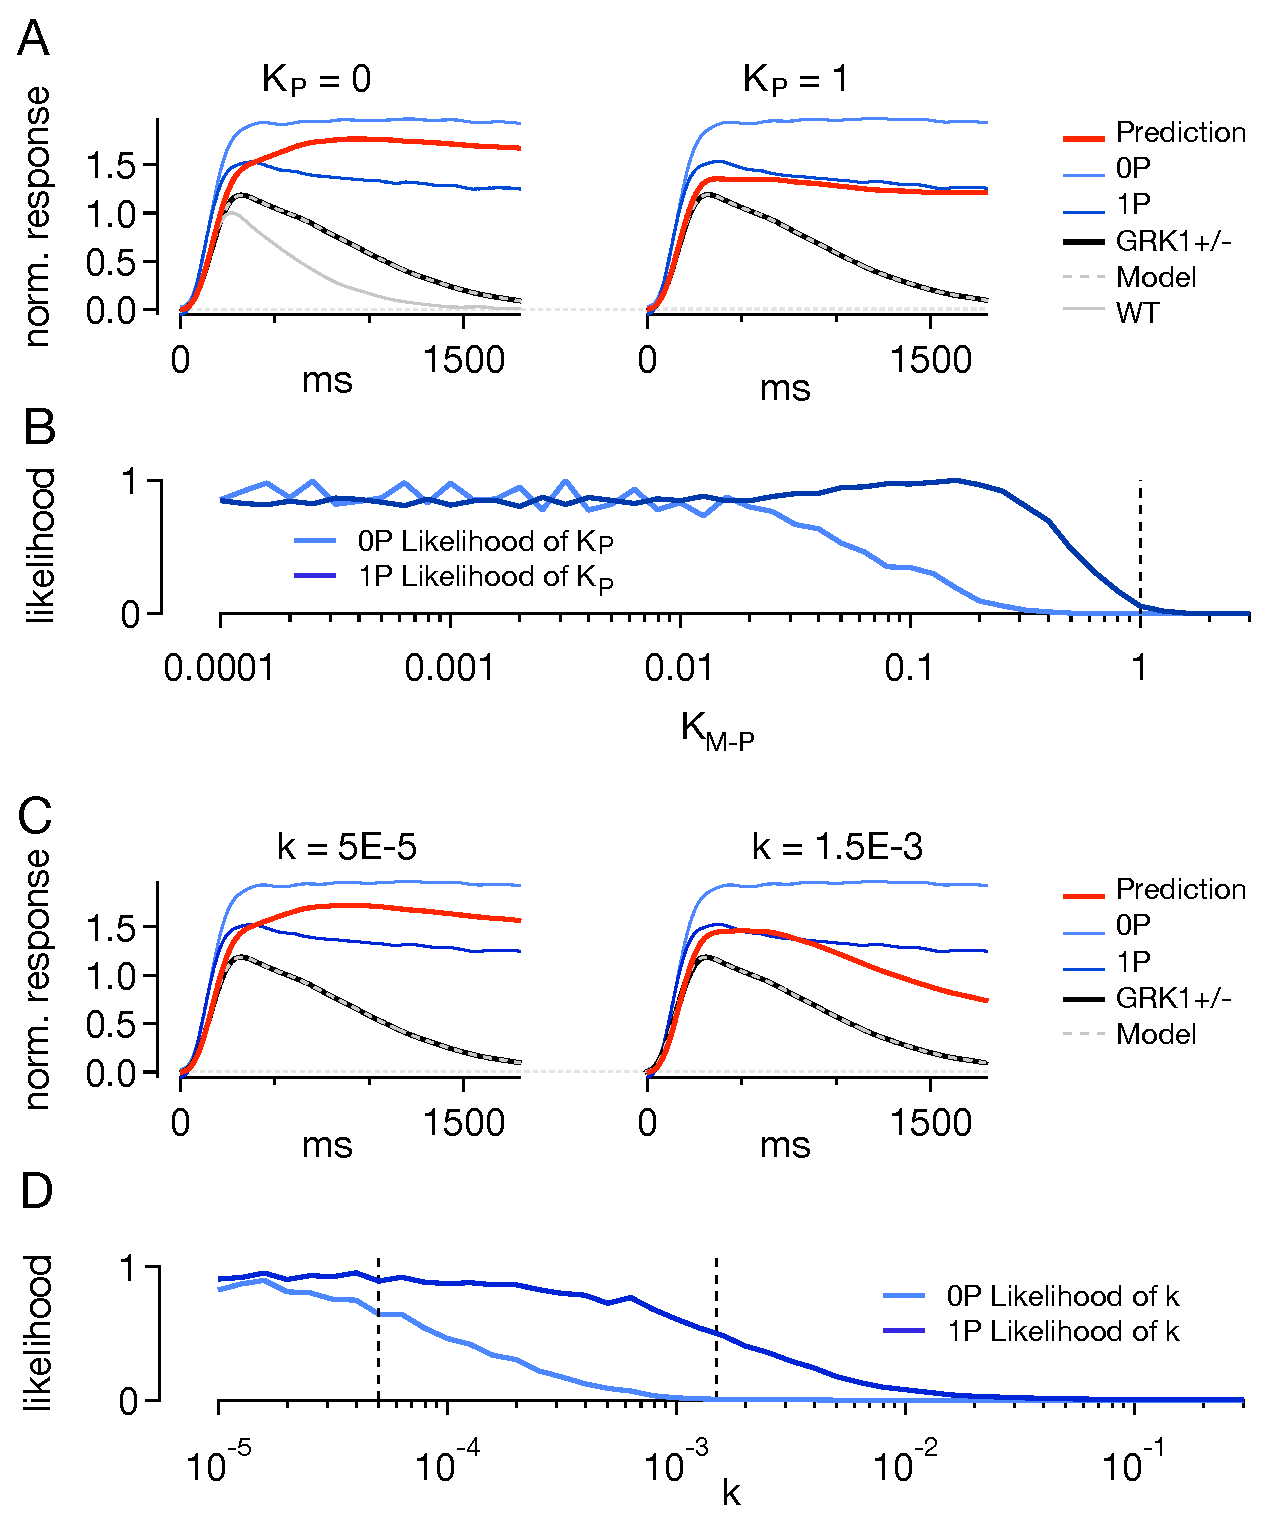
\includegraphics[scale=.64]{Linearity.eps}
\end{center}
\end{fullpage}
\end{figure}

We simulated \sRKHet~receptor activity with \Trh$=640$ ms, \Ns$=8$, and $\delta=1$, and modeled disk reactions as a deterministic process with $\tau_G=200$ ms (Fig.~\ref{fig:linearity}).  We varied forms of compression (\Kme, and $\kappa$) and calculated the average disk activity, $\bar{E}(t)$, as in Figure \ref{fig:eparams}.  We then calculated the impulse response function that provides a match to the average \sRKHet~response.  Both the experimental and the model average  are shown in Figure \ref{fig:linearity}A (model, grey dotted trace; \sRKHet, thick black trace), and are normalized to the average \sWT\ response (grey trace).  The filter and compression were then held constant while we altered rhodopsin parameters to simulate the mutant 0P activity (\Trh\ = 23.4 s, \Ns$=1$) \cite{Doan:2006jr}. 

Figure \ref{fig:linearity} compares the measured 0P responses (light blue) with those of \sRKHet~rods (trace black trace).  The mean single-photon response from normal rods is shown for comparison.  The predictions of the model are shown with thick red traces.  The predicted response without compressive effects is, if anything, slightly smaller than those measured (Fig.\ \ref{fig:linearity}A, left, \Kme\ $ =\kappa=0$).  Naturally, as compression increases, the amplitude of the model prediction decreases (Fig.~\ref{fig:linearity}A, right), and the likelihood also declines (Fig.~\ref{fig:linearity}B,D).

Mouse transgenesis can lead to varying amounts of protein expression \cite{Nagy:2003vv}.  For 0P and 1P rods, this can lead to random levels of rhodopsin expression, and may cause rods to compensate, possibly changing response kinetics \cite{Liang:2004hn}.  It was noted that 0P rods are shorter than \sWT\ rods, and it is possible that a decrease in length for 0P rods implies an accompanying decrease in plasma membrane surface (its width may also expand).  Rods expressing 0P rhodopsin have normal dark currents, so if the cGMP concentration remains the same in a smaller rod, the increased amplitude of 0P responses may be due to a higher density of channels \cite{Caruso:2010fe}.  As a control for this effect, we measured responses from rods expressing both WT and S338 (1P) forms of rhodopsin (the 0P line is no longer available).

\begin{figure}[htb]
\begin{center}
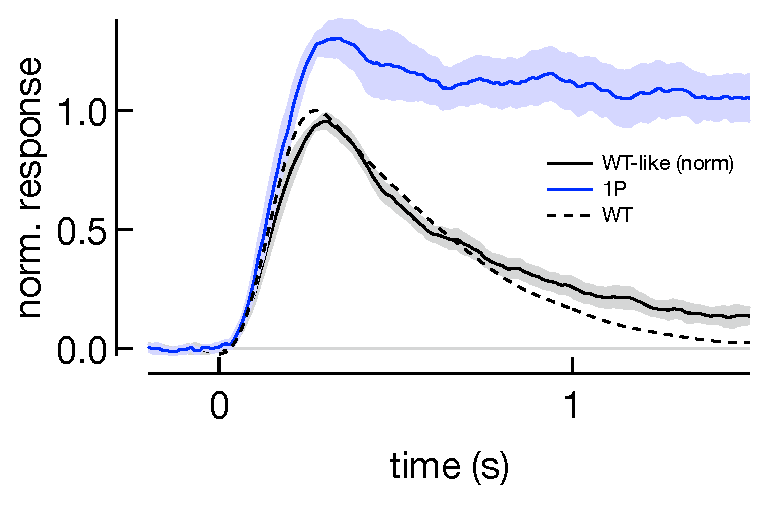
\includegraphics[scale = .45]{s338RhoHet.eps}
\caption[Responses in rods with 1P and WT rhodopsin co-expression.]{Responses in rods with 1P and WT rhodopsin co-expression at 30\textcelsius.  Responses from S338 (1P) rhodopsin could be distinguished by their prolonged activity (blue trace, $\pm$SEM).  Responses that are identified as originating from WT rhodopsin (black trace) show similar kinetics to responses recorded in rods of \sWT\ mice (dotted line).}
\label{fig:comborods}
\end{center}
\end{figure}

Responses to 1P activation were easily identified by their prolonged activity.  The resulting ensemble reached a larger amplitude on average than normal responses, similar to those reported in \OneP/\sRhoKO~ in our recording conditions \cite{Doan:2006jr}.  Figure \ref{fig:comborods} compares the results of these recordings with the average response in \sWT\ rods; the 1P response amplitudes are used in the analysis described below and in Figure \ref{fig:linearity}A,C (dark blue lines).  As previously observed, 1P response amplitudes are not as large as 0P responses,  though still larger than in \sRKHet rods (Fig.~\ref{fig:linearity}).  The reduction in amplitude was proposed to reflect fast phosphorylation of the single remaining site, reducing the rate of transducin activation \cite{Gibson:2000vf,Mendez:2000vh}.  

Regardless, we assume rhodopsin activity is step-like as above (\Trh\ = 18.8 s, \Ns$=1$) \cite{Doan:2006jr}, and ask whether compression of the cascade can account for the difference in S338 vs. \sRKHet amplitudes, and if so, for what range of values is likelihood high?  Figure \ref{fig:linearity} plots the probability of observing the mean S338 amplitude (when expressed along with normal rhodopsin) for a given set of parameters if the cascade is constrained to mimic the \sRKHet responses.  In this case, larger values of compression parameters become more likely, where eventually values of \Kme$>1$ lead to model predictions $>50$-fold less likely.  In particular, values of $\kappa$ appear to range further.  However, the right panel in (C) shows that even for values that provide a good match to the amplitude, as more PDE is activated and used up, less is available and the response begins to recover.  We conclude that this behavior makes this form of saturation unlikely and we focus below on the compression of disk activity (Eq.~\ref{eq:compr}).

Thus far, in Figures \ref{fig:linearity} and \ref{fig:comborods}, we have evaluated how well different models account for responses in mutants with prolonged receptor activity.  In doing so, we have shown that a linear cascade provides a likely explanation for mutant responses, but that models with some compression (\Kme$<1$) can also explain the data.  However, in the following sections we use additional features of experimental data to show that values of \Kme\ within the allowable range are unable to suppress variability in receptor activity.  In order to present this evidence, we first develop our method of evaluating particular model parameters and then investigate how different parameters control the model's behavior. 
  
\subsection{Constrained nonlinearities do not suppress variability in receptor activity}

Could the variability due to stochastic receptor activity, at the input to the cascade, be suppressed by the effects of compression acting downstream, within the range established by experiments in Figure \ref{fig:linearity}?
To address this question, we asked how well a set of parameters captured the total response variability (\CVarea), the time-to-peak of the variance relative to the mean response (\tpeakratio), and the width of the variance ($w_{\sigma^2}$) (see Fig.~\ref{fig:features}).

\begin{figure}[tb!]
\begin{center}
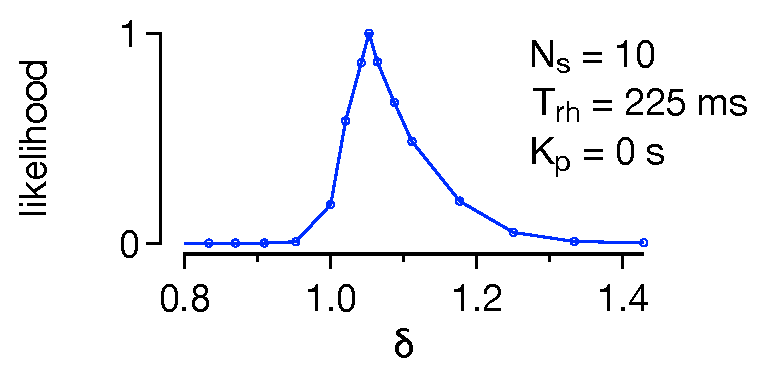
\includegraphics[scale=0.6]{deltaLikelihood.eps}
\caption[Likelihood estimates for reduction in rhodopsin activity.]
{Likelihood profile across parameter values governing reduction in rhodopsin activity (WT at 36C).  Other parameters were held fixed.
}
\label{fig:deltalikelihood}
\end{center}
\end{figure}

Figure \ref{fig:deltalikelihood} illustrates this approach for a linear cascade (\Ns$=10$, \Trh$=225$ ms, \Kme$=0$ s) while varying the parameter $\delta$.  We find that $\delta \sim 1$, in which case, average rhodopsin activity follows an exponential decay, with time constant \Trh.  We fix this parameter below to simplify the demonstration of model behavior as nonlinearities are included.  We then generated responses across a range of receptor lifetimes $25 \leq T_{Rh} \leq 325$ and shutoff steps, $3 \leq N_s \leq 12$, while also varying the compression of disk activity, $0 \leq $\Kme$\leq 5$.  Note, for illustration purposes, we have extended the range of compression beyond those suggested by the experiments of Figure \ref{fig:linearity}.

\begin{figure}[tb!]
\begin{center}
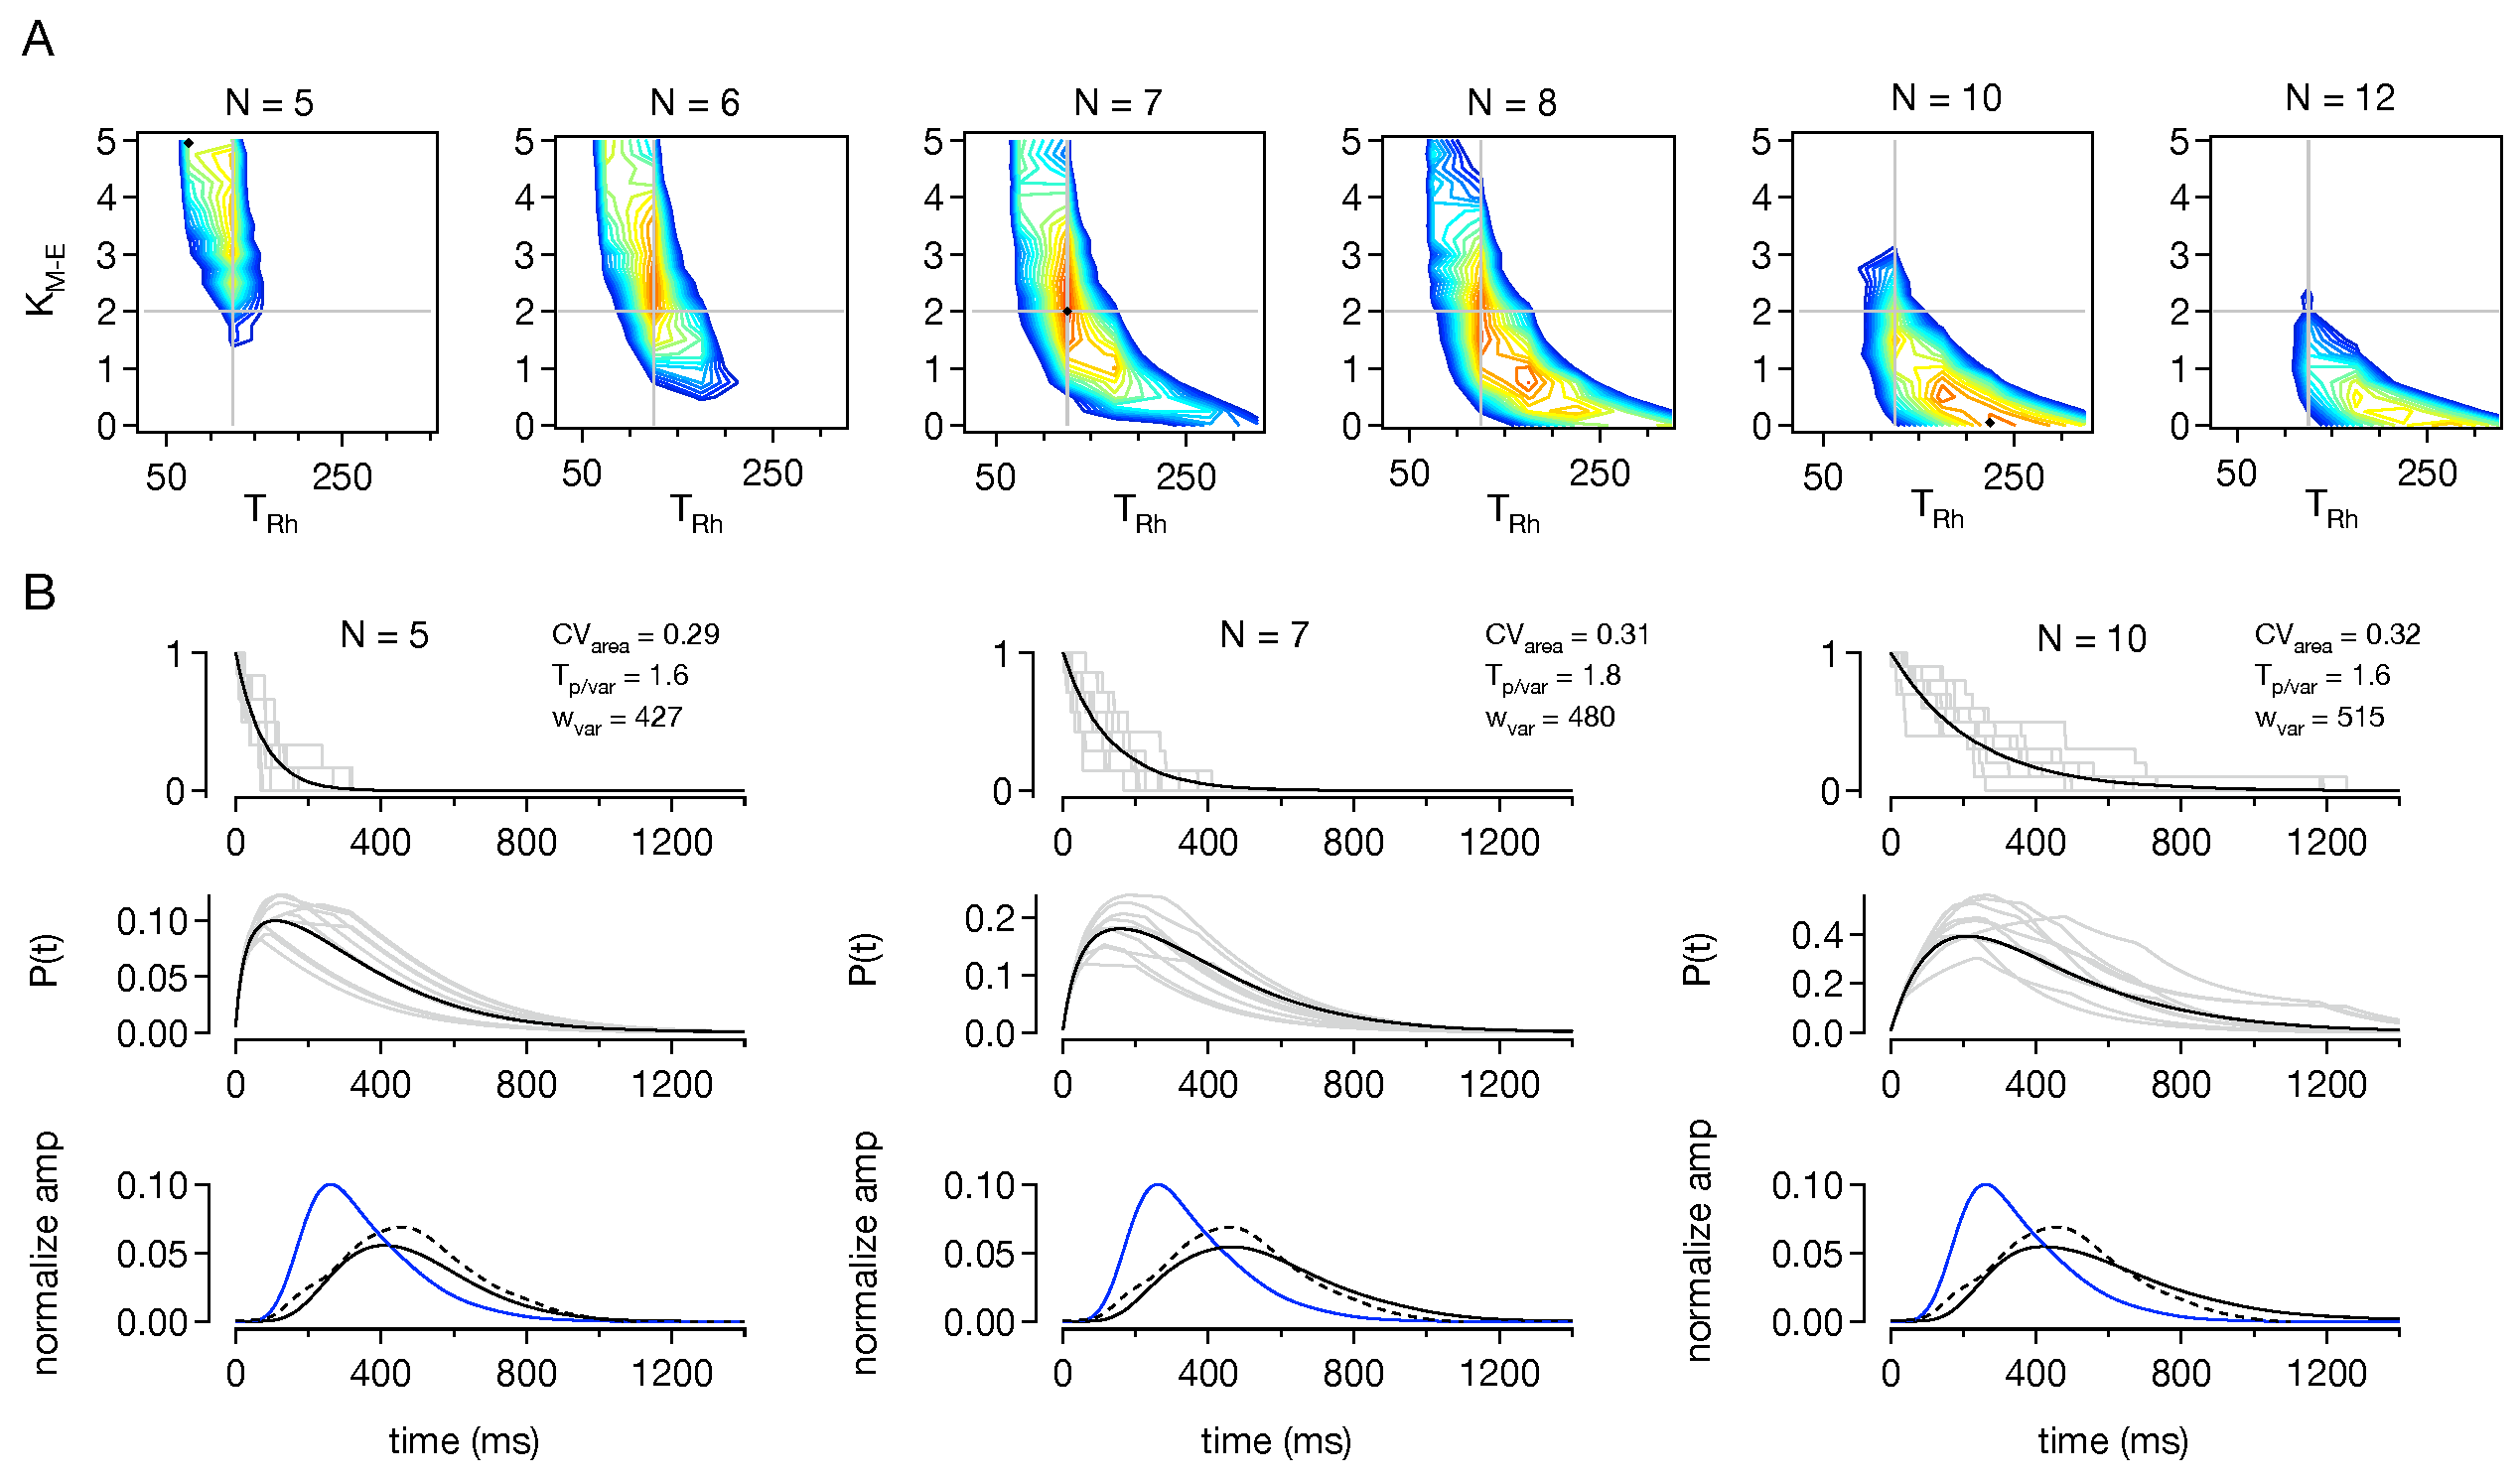
\includegraphics[scale=0.34]{ContoursSteps.eps}
\caption[Likelihood landscapes across parameters for \sWT\ rods: \Kme, \Trh, \Ns.]
{Likelihood landscapes across parameters, \Kme, \Trh, \Ns, compared to WT at 36C.
A)  Log-likelihood is plotted in contours (0.25 log units each), where green hues represent a reduction in likelihood of $\sim100$.  Grey lines plot maximum-likelihood estimates for the parameters \Kme\ and \Trh.
B) Example models for parameters represented as black diamonds in panels in A. Example trajectories are shown in grey, averages of 5000 simulated trajectories in black.  Note the different scales for $E(t)$ as compression changes.  Lower panels compare the model ensemble time-dependent variance (blue traces, right axes) with the experimentally measured variance (dotted blue traces, right axes). The two models on the left are not within the constraints of Figure \ref{fig:linearity}.
}
\label{Fig_Contours_WT36C}
\end{center}
\end{figure}

Figure \ref{Fig_Contours_WT36C}A plots contours of constant log-likelihood for values of compression, \Kme, and receptor decay time constant, \Trh, where the number of shutoff steps \Ns\ is held constant in each panel (shown above each panel).  The color scale is constant across panels, with red indicating likely parameters, and each contour line reflecting a $10^{1 \over 4}$ reduction in likelihood, such that the transition from green to blue reflects parameter values that are 100-fold less likely to represent the data, and violet indicates a factor of $10^{-4}$. Grey lines plot the maximum likelihood parameters for reference (\Ns$=7$, \Trh$ = 175$ ms, and \Kme$ = 2$), and as \Ns\ changes, the most likely values of \Trh\ and \Kme\ can be seen to drift.  

As we might naively expect, the likelihood landscapes show that nonlinear coupling of disk activity, $E(t)$, with the transduction filter can mitigate the effects of variability on the disk. First, as the number of steps decreases (leftward through panels), compression must increase to offset fewer steps (y-axis).  At the same time, the time constant of receptor decay also decreases (x-axis), until when \Ns$\leq7$,  \Trh$\sim125$ ms remains the most likely estimate.  The traces below help to illustrate model behavior by showing intermediate trajectories at each stage for the parameters indicated by the crosses in the panels above.  With few shutoff steps, substantial compression was required to reduce the variability to match experiment (Fig.~\ref{Fig_Contours_WT36C}B, left).  This compression decreases variability near the peak of the PDE activity, but not during the falling phase, hence pushing the variance to later times.  To counter this effect and match the measured time-to-peak of the variance, \Trh\ must be reduced. Conversely, a longer time constant ($\sim225$ ms) is required to account for this late variance when \Ns\ increases and compression is relieved.  These parameters trade smoothly and permit a large range of compressive effects: when $N_s=6$, a value of $K_E = 2.5$ is still highly likely.

Figure \ref{Fig_Contours_GCAP36C} depicts the same range of models evaluated for their ability to account for larger and slower single-photon responses in \sGCAP\ rods (at 37\textcelsius) which lack \Ca mediated acceleration of cGMP synthesis.  We would expect a common stochastic model for rhodopsin inactivation to account for responses in both \sWT~ and \sGCAP~ rods as knock-out of GCAP proteins should not affect any of the mechanisms involved in G protein activation or receptor desensitization.  In addition, experiments in which \Ca concentration in in \sGCAP~ rods is buffered with BAPTA suggest that changes in \Ca have little affect on the single-photon response except via control of cGMP synthesis \cite{Burns:2002un}.  If anything, we might expect that local cGMP concentration in the disk space would be replaced more slowly, thus exacerbating hydrolysis rate compression, \Kme.  This appears not to be the case; rather, we find generally the same trend as for \sWT, with higher values for suppression relatively less likely, but with consistent expectations for receptor kinetics.  

\begin{figure}[htb]
\begin{center}
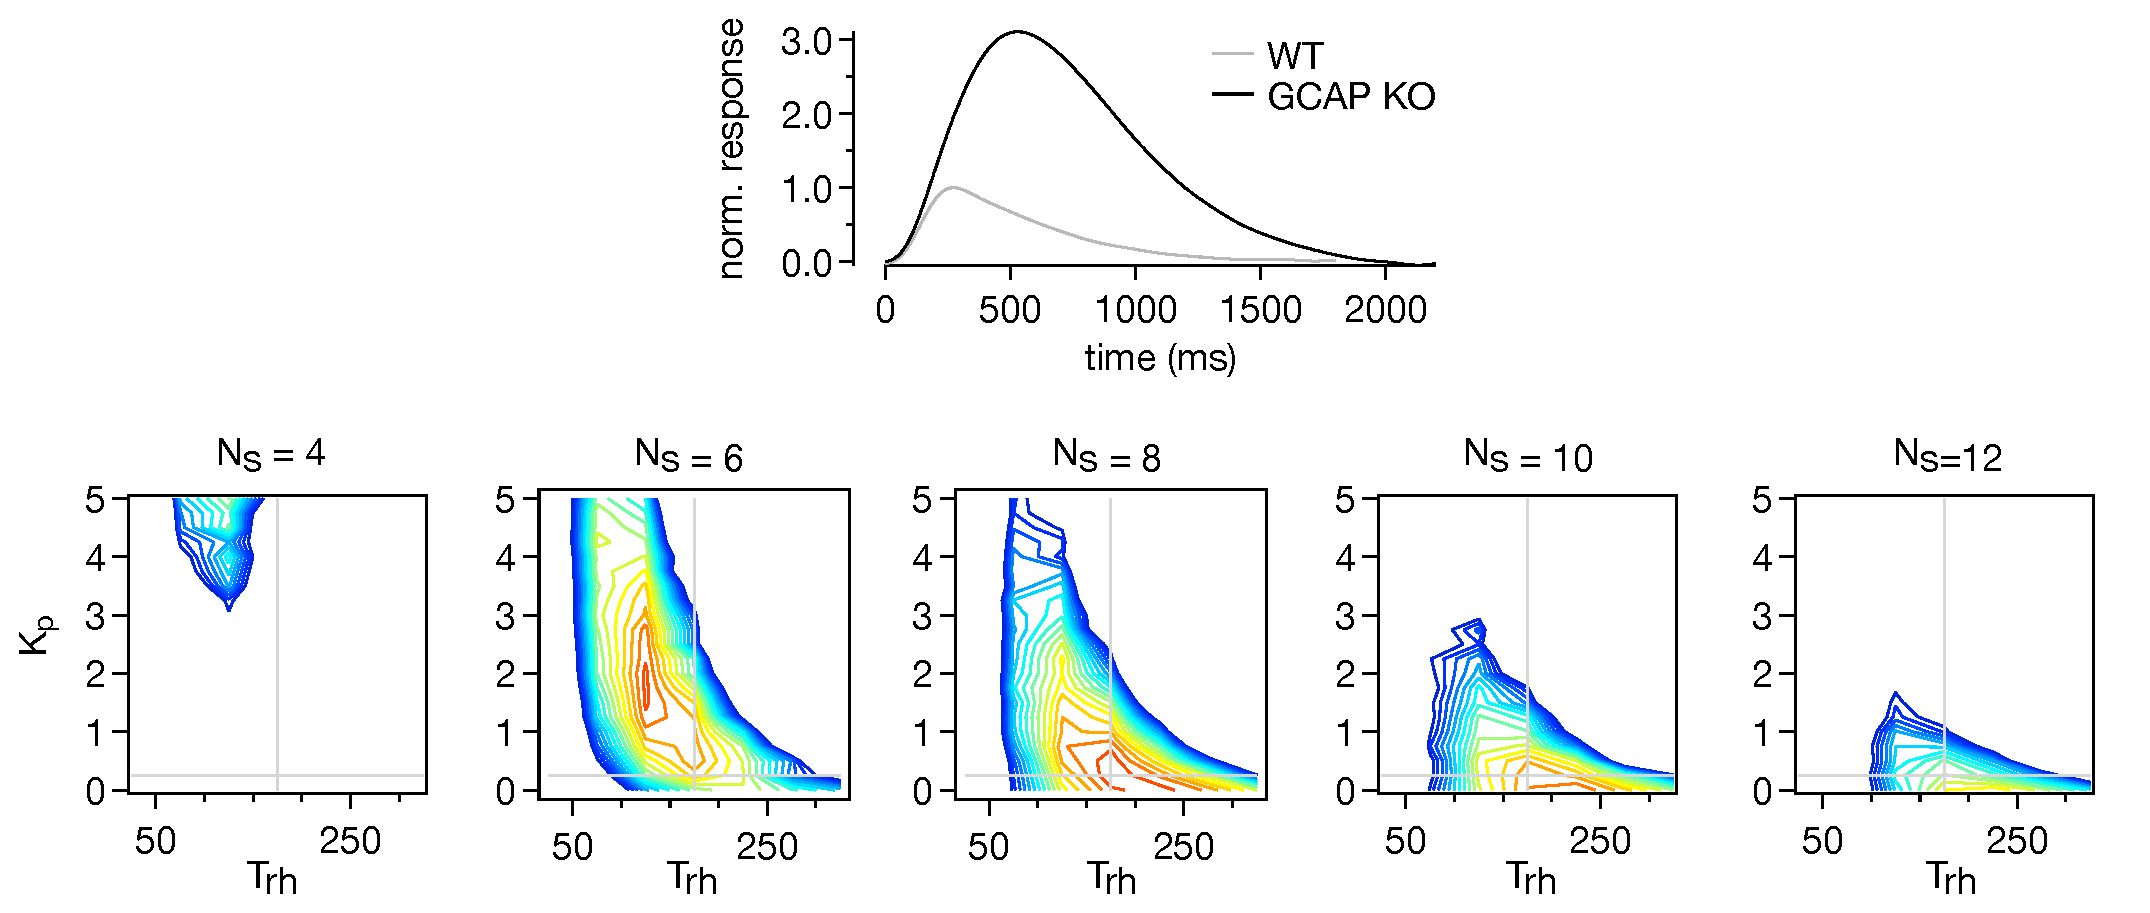
\includegraphics[scale=0.42]{ContoursStepsGCAP.eps}
\caption[Likelihood landscapes across parameters for \sGCAP rods: \Kme, \Trh, \Ns.]
{Likelihood landscapes across parameters, \Kme, \Trh, \Ns, for models of \sGCAP responses at 37\textcelsius.
A) Average single-photon responses of \sWT\ (grey) and \sGCAP\ (black) rods.  Responses are normalized for comparison with Fig.~\ref{fig:linearity}.
B)  Log-likelihood is plotted in contours (0.25 log units each), where green hues thus represent a reduction in likelihood of $\sim100$.  Grey lines plot most likely values for the three parameters.
%B) Example models for parameters represented as diamonds in panels in A.
}
\label{Fig_Contours_GCAP36C}
\end{center}
\end{figure}

Finally, we return to our initial question of whether nonlinearities permitted by the comparison between \sRKHet and 0P responses (Fig.~\ref{fig:linearity}) can offset variability introduced by stochastic receptor activity.  Compression values \Kme$>0.5$ failed to capture the amplitude of 0P and 1P responses.  By reviewing the contour plots in Figures \ref{Fig_Contours_WT36C} and \ref{Fig_Contours_WT36C}, we can see that if \Kme\ is restricted to values within this range, then the data are best explained by rhodopsin inactivation requiring 8-11 steps with a \Trh\ of $175-250$ ms in both \sWT\ and \sGCAP\ rods.  Over this range, then, compression is does not dramatically alter the characteristics of the single-photon response variance, implying that reproducibility of the single-photon response directly reflects reproducible receptor activity.

\subsubsection{Consequences of a linear cascade}

A linear cascade allows an intuitive explanation for the dependence of likelihood on various parameters.  For linear models, \CVa\ is controlled entirely by the number of inactivation steps and hence directly constrains this parameter.  The \tpeakratio depends primarily on the duration of rhodopsin's activity relative to the kinetics of the transduction cascade filter, with a weak dependence on the number of steps.  Finally the width of the variance is primarily determined by how much activity declines following each step; with little decline following each step, the variability all occurs in a narrow window following the final decay step, whereas with a distribution of decay across steps, variability is more spread out over time.

\subsubsection{Possible sources of variability}

We have chosen stochastic fluctuations in receptor activity to be the source of trial-to-trial variability in our model.  In reality, the number of activated transducin or PDE molecules is also stochastic, which we have avoided including here.  To see the implication of this choice consider a linear cascade process, such that additional activity at any point in the cascade causes a proportional change in the current.  Regardless of its kinetic properties, a linear cascade does not change the coefficient of variation of the single-photon response area.  If rhodopsin is the sole source of variability, then coefficient of variation of the current area is identical to the coefficient of variation of rhodopsin's integrated or cumulative activity.  Intuitively, this equality originates because the relation between the area of a given rhodopsin trajectory and the current is given by the area of the linear transduction filter --- i.e. a single scalar number.  This scale factor affects the mean and standard deviation of the responses equally and will not change the coefficient of variation.  The \CVa\ is then an upper bound on trial-to-trial variation in rhodopsin activity, and if we were to model transducin activity as stochastic, rhodopsin inactivation would have to be even more tightly controlled to produce the low \CVa\ that we observe experimentally.  Thus, in the simple multi-step shutoff model here, rhodopsin inactivation would require a minimum of 8 to 11 steps to explain the measured \CVa\ of 0.3 to 0.35 (i.e. \CVarea$= 1/\sqrt{N_s}$). 

\section{Discussion}

Rod phototransduction presents a unique opportunity to explore enzyme cascades and GPCR mediated signaling quantitatively.  Here, we use the characteristics of ensembles of isolated single-photon responses to explore the behavior of a simple model for coupling the activity of the GPCR rhodopsin to the rod outer-segment current, and compare across normal mice and a number of transgenic lines.  Our results show that explaining response properties across a number of genetic lines requires a cascade that effectively acts linearly on the receptor throughout its active lifetime.  Consequently, the low variability of the single-photon response provides an upper bound on variability in receptor activity and thus implies tight regulation of the total receptor activity.  Spreading total activity across multiple steps, each with first order kinetics, provides an efficient description of a process with low intrinsic variability, and in this context, rhodopsin desensitization requires at least 8 steps and a time constant of $\sim225$ ms.

\subsection{Multi-step models of rhodopsin desensitization}

The low variability of single-photon response ensembles has provided a valuable target for models of phototransduction reaction dynamics, and as such these higher order characteristics have inspired efforts to identify their origin, first in amphibian rods \cite{Rieke:1998hx,Whitlock:1999wm,Hamer:2003gc,Hamer:2005ec} and subsequently in mammalian rods \cite{Mendez:2000vh,Field:2002vf,Doan:2006jr,Doan:2009jq}.    Experiments and modeling in amphibian rods suggest that rhodopsin desensitization is tightly regulated to introduce low variability in the number of active transducin molecules across responses.  Molecular properties are not as well measured in mammalian rods, prompting the use of signatures of the time-dependent variance to constrain models, the approach adopted here for mouse rods \cite{Field:2002vf}.  In past work, models of feedback to rhodopsin were ruled out because they produced ensemble variance that was very narrow in time, similar to receptor activity that abruptly terminates in this study.  Multi-step models of gradual receptor inactivation required a large number of steps to explain the low variability of primate and guinea pig single-photon responses, on order $\sim12-14$, and an additional model for component exhaustion could reduce this requirement.

A potential source of this regulation is the inactivating steps of phosphorylation and arrestin binding.  Genetic ablation of GRK1, the substrate phosphorylation sites, or arrestin1 severely disrupt response recovery \cite{Chen:1995td,Chen:1999tp,Xu:1997dp}, while substitution of alanine for subsets of phosphorylation sites reveal a range of resulting response characteristics \cite{Mendez:2003tf}.  Prevailing experimental techniques initially prevented isolation of single-photon responses and, consequently, the characterization of their variance, but overcoming this limitation further revealed the importance of the full complement of sites in keeping the coefficient of variation of response area low \cite{Doan:2006jr}.  The sensitivity of the \CVa\ to removal of a single phosphorylation site is suggestive that variation in receptor activity translates effectively linearly to fluctuations in the outer segment membrane current.  The approach presented here hypothesizes linear models for receptor and cascade but also tests the ability of two nonlinear mechanisms to mask additional receptor variability.

\subsection{Non-linear mechanisms controlling variability}

Non-linear mechanisms are recruited to expand the regime of illumination over which the rod can respond, and are critical for adaptation to light intensities above darkness \cite{Fain:2001uo,Koutalos:1996ue}.  
The models of mammalian phototransduction discussed thus far use a linearized version of cascade reaction equations, perhaps an oversimplification.  A further simplification is to ignore the specialized rod morphology and the limitations to diffusion that it potentially creates.  The extension of models to include these considerations have raised the possibility that spatial-temporal restriction of second messengers could create nonlinear relationships between cascade elements that could reduce variability in receptor activity \cite{Andreucci:2003fq}.  In particular, it appears that the tortuous geometry could prevent cGMP diffusion and enhance local depletion in the inter-disk volume by PDE hydrolysis, reducing the effectiveness of additional PDE \cite{Caruso:2011fv,Bisegna:2008dc}.  These models indicate that cooperative channel gating and \Ca dependent feedback may also act to reduce variability, but experimental evidence suggests their effect is limited \cite{Burns:2002un,Field:2002vf}.

%While intriguing and detailed, these studies match the kinetics of the model to those of responses recorded under different conditions than the isolated unitary responses used as constraints here.  The difference in kinetics between the experimental protocols is significant, and in particular, as alluded to above, the alternate recording conditions also prevent measuring single-photon responses, let alone characterizing their variance \cite{Azevedo:2011ev}.  Thus, in comparing characteristics across protocols, the relevance of these studies may be limited.  These detailed mechanistic models also implicate nonlinear mechanisms in channel activation and \Ca feedback to guanylyl cyclase.  This may also reflect a constraint imposed by the average kinetics the model is forced to replicate, as experimental evidence suggests their effect is limited \cite{Burns:2002un,Field:2002vf}.

Nevertheless, these studies emphasize the possible impact of compression, and we tested this possibility here.  As predicted, increasing compression relaxes constraints on receptor inactivation, and the number of steps required to control activity can decrease as a result (Fig.~\ref{Fig_Contours_WT36C}.  This trade-off is necessarily accompanied by a faster decay in receptor activity.  However, the degree of compression that permits significant reduction in the number of inactivation steps also appears to be incompatible with increased disk activity produced by 1P and 0P mutant receptors.  

Models that incorporate the geometry of the rod also suggest that these responses can be affected by changes in rod volume brought on by transgenic expression \cite{Caruso:2010fe}.  However, tandem expression of the 1P mutant receptor along with WT rhodopsin shows that even in rods which exhibit normal kinetics for wild-type responses, the mutant response amplitudes are increased, consistent with results from ectopic expression of rhodopsin mutants lacking a C-terminus \cite{Chen:1995td}.

%\subsection{Additional sources of variability}
%
%We conclude that during elementary responses in darkness, the mouse rod transduction cascade is effectively linear, implying an inability to remove variance.  As we have chosen to model a single source of variability, the \CVa\ sets an upper bound on the intrinsic variability of the receptor, and additional stochastic activity would place yet further constraints on rhodopsin.  The reactions coupling the transduction of receptor activity to outer segment current involve stochastic activity at each stage \cite{Detwiler:2000de}.  In the case of small perturbations, while each stage may be expected to respond linearly on average, the small number of molecules involved might imply large trial-to-trial variation in their number \cite{Hamer:2003gc}.  
%
%Although variability introduced by rhodopsin and transducin can have similar effects on \CVarea, they have different effects on the shape of the time-dependent variance.  Linear models in which variability is dominated by transducin activation fail to capture the late variance, unlike those in which rhodopsin inactivation dominates.  This occurs because variability then tracks transducin activity. The inability of fluctuations associated with transducin activation to capture the late peak of the variance observed in experiments remains across a wide range of relative durations of rhodopsin and transducin activity.  

\subsection{Mechanism of steps}

The multi-step shutoff model for rhodopsin inactivation presented here is attractive for its tractable implementation, its simple set of parameters, and for the general picture of desensitization kinetics it provides.  Such models use the number of steps simply as a proxy for total variability: the steps are modeled as first order random processes such that the integrated activity is effectively the sum over the random, Poisson activity of each step \cite{Rieke:1998hx,Field:2002vf,Doan:2006jr}.  This model has been a concise way to generate hypotheses and to drive continual investigation of mechanisms that control single-photon response kinetics, though the molecular mechanisms proposed to support this low variability have changed as hypotheses have been tested.  

Phosphorylation of the receptor appears an important contributor of mechanisms reducing variability.  Biochemical experiments suggest that while multiple-phosphorylation is possible \cite{Wilden:1982ur}, that not all phosphorylation sites are necessary for tight arrestin binding, or that some play more important roles than others \cite{Kennedy:2001us,Maeda:2003um,Vishnivetskiy:2007ip}.  Meanwhile, mutations of phosphorylation sites indicate both the possibility for complete phosphorylation \emph{in vivo}, as well as the importance of the full complement of phosphorylation sites \cite{Mendez:2003tf,Doan:2006jr}.  It is possible that different complements of sites contribute in specific ways, such that not all phosphorylation events are equivalent \cite{Brannock:1999cz}, and particular sites may act as important structural features mediating interactions with GRK1 or arrestin1 rather than as substrates for phosphorylation \cite{Kisselev:2004ii}.    The outer-segment concentrations of arrestin1 and GRK1 also play a role, likely through competition for rhodopsin; steps could then represent the composite of multiple reactions \cite{Doan:2009jq}.  

As a more detailed picture of rhodopsin desensitization emerges, it will have to account for low ensemble variability.  The approach presented here provides a framework for testing future models against experimental data.

%\bibliographystyle{jneurosci}
%\bibliographystyle{plain}
%\bibliography{rho_phosp_biblio}

%\end{document}



%Round up results
%State most likely arrangements, with confidence intervals (eg 2 likelihood log units)
%	Consequences of linearity: variation cannot be eliminated, need for regulated rhodopsin 	desensitization.
%Review model from Tranchina.  Discuss Caruso model in this context, StoA is a nice test of their explicit prediction that StoA and WT are essentially identical, with slower kinetics.  Once they turn off modules (diffusion, feedback, etc), both StoA and WT do essentially the same thing.
%
%Limitations of this study: how does the constraint of filtering to get average response impact our estimates?  No mechanistic details of how compression (however limited it might be) might work, and still no mechanistic understanding of source of steps (Thuy�s model still best).
%
%


%\leftline{\bf Todo: analysis/conceptual}
%
%
%%Table of parameters?
%\be
%\i{Rh - Tau, Nsteps, delta, compression Rationale for multiple step representation of rhodopsin}
%\i{T - base rate, tau (200 ms), TransRateCompression, TransCompression (exhaustion)}
%\i{Compression of either, both, different kinds: rate compression vs exhaustion of resources}
%\i{Compression of response (haven�t used yet).}
%\ee

%%The coupling between rhodopsin and transducin could in principle be affected by local depletion of transducin, for which steady state is reached as transducin decay replenishes the concentration \cite{Felber}. We model this as a Michaelis relationship for rhodopsin rate where:
%\begin{equation} 
%Rh = \frac{Rh}{1+K_{M-R} Rh}.
%\end{equation}
%We find, however that this effect is similar to alterations in the parameter $\delta$ describing step decay and avoid descriptions of its influence in the results.
%\be
%
%\i{We are ignoring feedback --- is this ok?}
%
%\i{Can we ignore saturation at channels?  There seems to be decent evidence against it, and it is hard to cleanly implement.}
%
%\i{Clarify argument about \CVa\ for stochastic transducin model in methods --- some of this can be taken from Dan's notes on subject.  Make sure consistent with how simulations are being done.}
%
%\i{Decide how many different saturation models to consider: (1) Rh; (2) cumulative T; (3) instantaneous transducin}
%
%\i{Run likelihood models for various combinations of noise from rhodopsin and transducin}
%
%\i{How do we handle Rh* inactivation time constant in cases where inactivation not exponential?}
%
%\i{Make schematic figure showing parameters used from time-dependent variance}
%
%\i{Other comparisons for likelihood analysis?}
%
%\i{Add table with experimental parameters and model results}
%
%\i{Include more raw \sGCAP\ data since that is new}
%
%\i{How biased are single-photon responses - i.e. are these cells out of the norm?  Check Pepperberg time constants if we have them on cells from which we have isolated singles.  Any other parameters too.}
%
%\i{GCAP knockout feedback analysis}
%
%\i{wt/1P comparison with coexpression}
%
%\i{A version of the model that explores parameters of Rh compression or T compression for both $tau_Rh \, \sim600$ ms and a step of rhodopsin activity}
%
%\i{Hopefully this range is small enough not to affect the variability constraints}
%\i{T exhaustion so far doesn�t seem too likely}
%
%\i{I found for WT36C that a moderate rate compression of T was likely, ~.008 at T rate of .5 (p =1/2 per time bin that a T gets activated).  Assumed ~50 T are activated by 100 ms, then .008*50 = .4 and compression is ~1/1.4}
%
%\i{normalize compression ratios so that they don�t depend on activation rates and mean something by themselves}
%
%\ee
%




%Goal: assess the likelihood of a given model for single-photon responses based on a collection of experimental responses.  Use this approach to determine most likely model parameters (e.g. trajectory of Rh* activity, degree of saturation in cascade, number of shutoff steps, ...). 

%This could be done in (at least) two broad ways: (1) use simulation of large collection of responses to characterize probability of observing a given response from model, and evaluate likelihood of each experimental response using this characterization; (2) use mean and SEM of parameters of response from experiment and use these to evaluate likelihood of given set of simulated responses.  In principle, option (1) seems preferable because it does not involve any assumptions about what matters about responses, and because measured responses can be evaluated against a large set of simulated responses (as large as needed to eliminate finite sample size effects).  In practice, however, this approach seems difficult for reasons given below.
%
%Consider a set of measured single-photon responses $r_n(t)$, which consist of a single-photon response with added continuous noise.  We can write these responses compactly as 
%\begin{equation}
%r_n(t) = \sum_i a_{i,n} e_i(t) + \eta(t)
%\end{equation}
%where $a_{i,n}$ are weights specific to response $n$, $e_i$ are a set of basis functions shared by all $r_n$ (e.g. principle components), and $\eta$ represents continuous dark noise.  We want to compare these to a set of simulated responses $s_n(t)$:
%\begin{equation}
%s_n(t) = \sum_i b_{i,n} e_i(t) 
%\end{equation}
%where $e_i$ are the same as those for the measured responses.  
%
%The ideal approach would seem to be to use the simulated responses to generate distributions $P(b_{i,n})$.  These distributions could then be used to evaluate the likelihood of each measured single-photon response --- i.e. the likelihood of $a_{i,n}$ for each single-photon response.  Combining likelihoods across all measured single-photon responses would tell us how likely a given set of measured responses is given a particular model.  We could then search across model parameters to find those that maximize the likelihood.  
%
%A problem with this approach is that we cannot obtain the $a_{i,n}$ directly because we cannot separate, on a single trial, the single-photon response and the continuous noise.  It would seem we are limited to making this separation on average, when we do not need to know the noise trajectory but instead only its covariance (or other statistics).  Thus we can estimate the distribution $P(a_{i,n})$ by projecting both single-photon responses and failures along each $e_i$ and correcting the single-photon response projections for that failures projections (e.g. if we assume things are gaussian we can subtract the variances).  This seems to preclude evaluating the likelihood of individual experimental responses against a set of simulated responses.
%
%One alternative would seem to switch things around --- evaluate the likelihood of individual simulated responses against the set of measured responses.  There are several issues with this approach.  One is whether we have a sufficient number of experimental responses to really estimate the full distributions (i.e. $P(a_{i,n}$).  Another more fundamental issue is that maximizing the likelihood of the simulated responses can be achieved by placing each response at the peak of $P(a_{i,n})$ --- i.e. removing all variability in the simulated responses.  
%
%The issues above would appear to complicate approaches based on single responses. 

%An alternative is to evaluate likelihood based on several parameters of the collected responses.  Those parameters could be the distributions of coefficients $P(a_{i,n})$ and $P(b_{i,n})$ or other quantities such as CV$_{area}$, $t_{peak, \sigma^2} / t_{peak, \mu}$, ... .  We can estimate the mean and SEM of these parameters from experiment (e.g. estimate each parameter for each rod and take mean and SEM of those estimates).  Then we can use the mean and SEM of each parameters to evaluate likelihood of given set of simulated responses.  This approach in practice seems to work quite well (meaning likelihood changes substantially for 10-20\% changes in model parameters).  



%Practical issues: we can collect a few thousand single-photon responses and a few thousand failures.  These come from 10-20 rods.  Responses of different rods differ in amplitude and kinetics, and in addition the properties of the dark noise vary from rod to rod.  Some, but not all, of this rod-to-rod variation can be eliminated by normalizing the peak amplitude and time to peak of the single-photon response to 1 before combining data across rods.  
%
%8/30/2011 FMR
%
%Here's another possibility.  Use PCA to identify low dimensional representation of combined experimental single-photon responses.  For each cell measure how much of total variability of single-photon responses is captured by each dimension.  Use these fractional variance measures, along with total variance (CV) in likelihood analysis.  

%%%%%%%%%%%%%%%%%%%%%%%%%%%%%%%%%%%%%%%%%
%
%\bigskip
%\noindent
%NOTES:
%
%\bi
%
%\i{should wt data be included in above?  Requires assuming something about rhodopsin time constant - or that could be backed out of data by deconvolving filter from measured response.}
%
%\i{try to replicate results with spatio-temporal diffusion model?}
%
%\i{analyze \sGCAP\ single-photon response and noise re linearity, add to this section.}
%
%\i{rgs9 overexpressors could test for saturation by decreasing transducin activity - would expect increase in CV if compression at PDE}
%
%\ei

%(Should we get quantitative?).
%\begin{equation}
%\langle q \rangle = \langle \lambda R^* \rangle = \lambda \langle  R^* \rangle
%\end{equation}
%\begin{equation}
%\langle (q -  \langle q \rangle)^2 \rangle = \langle (\lambda R^* - \lambda \langle  R^* \rangle)^2 \rangle = \lambda^2 \langle ( R^* - \langle  R^* \rangle)^2 \rangle, 
%\end{equation}
%such that
%\begin{equation}
% CV_{area}^2 = \frac{\langle (q -  \langle q \rangle)^2 \rangle}{\langle q \rangle^2} = \frac{\lambda ^2 \langle (R^* -\langle  R^* \rangle)^2 \rangle}{\lambda^2 \langle  R^* \rangle^2} = CV_{R*}^2.
%\end{equation}
%In this study, we model transducin activation is as a deterministic linear filter described by an exponential decay (Fig \ref{fig:rhparams}A), the time course of which is well-constrained in the range $\sim 200-250 ms$ \cite{Krispel}.  Theoretical considerations of multi-step models, together with stochastic transducin activation, predict that if an average $n_T$ transducin activations are spread across $N_s$ steps, then \CVarea$ = \sqrt{{1 \over N_s} + {2 \over n_T}}$.  Figure~\ref{fig:theory-limits} plots the dependence of \CVa\ on $n_T$ for several choices of $N_s$, where the dashed line plots the measured \CVarea.  If the current responds linearly to the number of transducin, allowable values of $n_T$ and \Ns\ fall below the dashed line.  Assigning variability to the receptor alone thus implies a lower bound on \Ns\ under certain circumstances.  The approach to evaluating cascade models introduced here will be useful to assess the implications of stochastic transducin activation in future models.  
%
%\begin{figure}[h]
%\begin{center}
%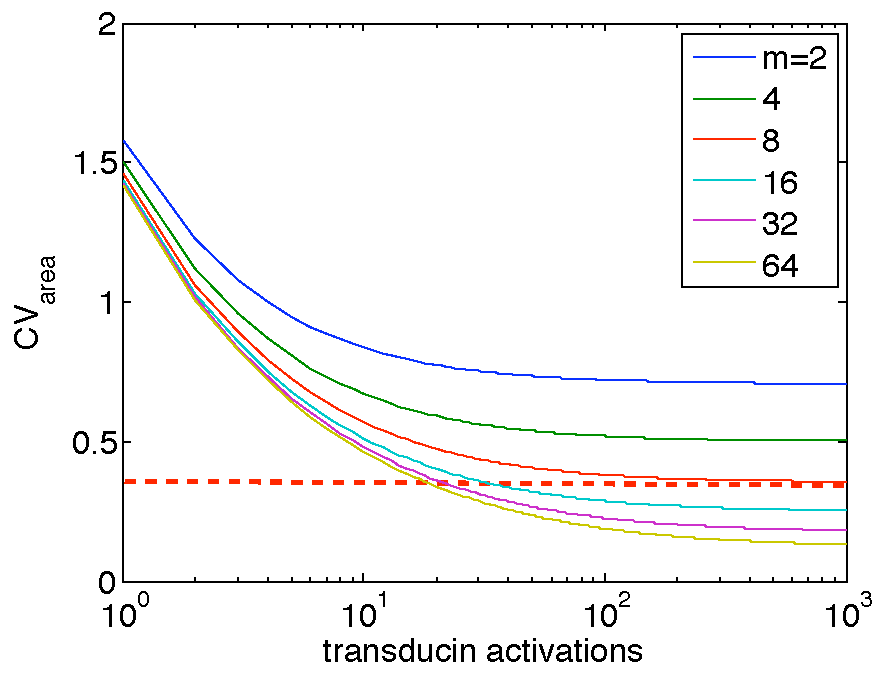
\includegraphics[width=3in]{theory-limits.pdf}
%\caption{Predicted \CVa\ as number of steps in rhodopsin shutoff and number of transducin activations are varied.  Dashed red limit plots measured \CVarea.}  
%\label{fig:theory-limits}
%\end{center}
%\end{figure}
